\section{Results}

\subsection{Variation in observed hospital thrombolysis use}

Thrombolysis use in the original data varied between hospitals from 1.5\% to 24.3\% of all patients, and 7.3\% to 49.7\% of patients arriving within 4 hours of known (precise or estimated) stroke onset.

%%%%%%%%%%%%%%%%%%%%%%%%%%%%%%%%%%%%%%%%%%%%%%%%%%%%%%%%%%%%%%%%%%%%%%%%

\subsection{Feature selection}

The best model with 1, 2, 5, 10, 25 \& all 60 original features had ROC AUCs of 0.715, 0.792, 0.891, 0.919, 0.923 \& 0.922. We selected 10 features for all subsequent work, which were:

\begin{itemize}
    \item \emph{Arrival-to-scan time}: Time from arrival at hospital to scan (mins)
    \item \emph{Infarction}: Stroke type (1 = infarction, 0 = haemorrhage)
    \item \emph{Stroke severity}: National Institutes of Health Stroke Scale (NIHSS) score on arrival
    \item \emph{Precise onset time}: Onset time (1 = precise, 0 = best estimate)
    \item \emph{Prior disability level}: Disability level (modified Rankin Scale; mRS) before stroke
    \item \emph{Stroke team}: Stroke team attended (hospital identifier)
    \item \emph{Use of anticoagulants}: Use of prior anticoagulant (1 = Yes, 0 = No)
    \item \emph{Onset-to-arrival time}: Time from onset of stroke to arrival at hospital (mins)
    \item \emph{Onset during sleep}: Did stroke occur in sleep?
    \item \emph{Age}: Age (as midpoint of 5 year age bands)
\end{itemize}

These were not necessarily the 10 most important features, as another highly correlated feature may also have been important, but if a feature is highly correlated with an already chosen feature, it will add less additional value.

Correlations between the 10 features were measured using coefficients of determination (r-squared). All r-squared were less than 0.05 except 1. age and prior disability level (r-squared 0.146), and 2. onset during sleep and precise onset time (r-squared 0.078).

%%%%%%%%%%%%%%%%%%%%%%%%%%%%%%%%%%%%%%%%%%%%%%%%%%%%%%%%%%%%%%%%%%%%%%%%

\subsubsection{Model accuracy}

Model accuracy was measured using stratified 5-fold cross validation. Overall accuracy was 85.0\% (83.9\% sensitivity and specificity could be achieved simultaneously). The ROC AUC was 0.918. The model predicted hospital thrombolysis use at each hospital with very good accuracy (r-squared = 0.977).

The appendix contains further model accuracy analysis (including patient subgroup analysis).

%%%%%%%%%%%%%%%%%%%%%%%%%%%%%%%%%%%%%%%%%%%%%%%%%%%%%%%%%%%%%%%%%%%%%%%%

\subsection{Characteristics of the most thrombolysable patient (at each hospital)}

As seen in Figure \ref{fig:results_most_thrombolysable}, compared with the other groups, the 132 most thrombolysable patients had:
\begin{itemize}
    \item shorter arrival-to-scan times
    \item an infarction stroke type
    \item moderate to severe stroke severity with NIHSS 5-25
    \item a precise onset time
    \item lower pre-stroke disability
    \item were not taking anticoagulant medication
    \item shorter onset-to-arrival times
    \item did not have onset during sleep
    \item were younger
\end{itemize}

\begin{figure}[!h]
\centering
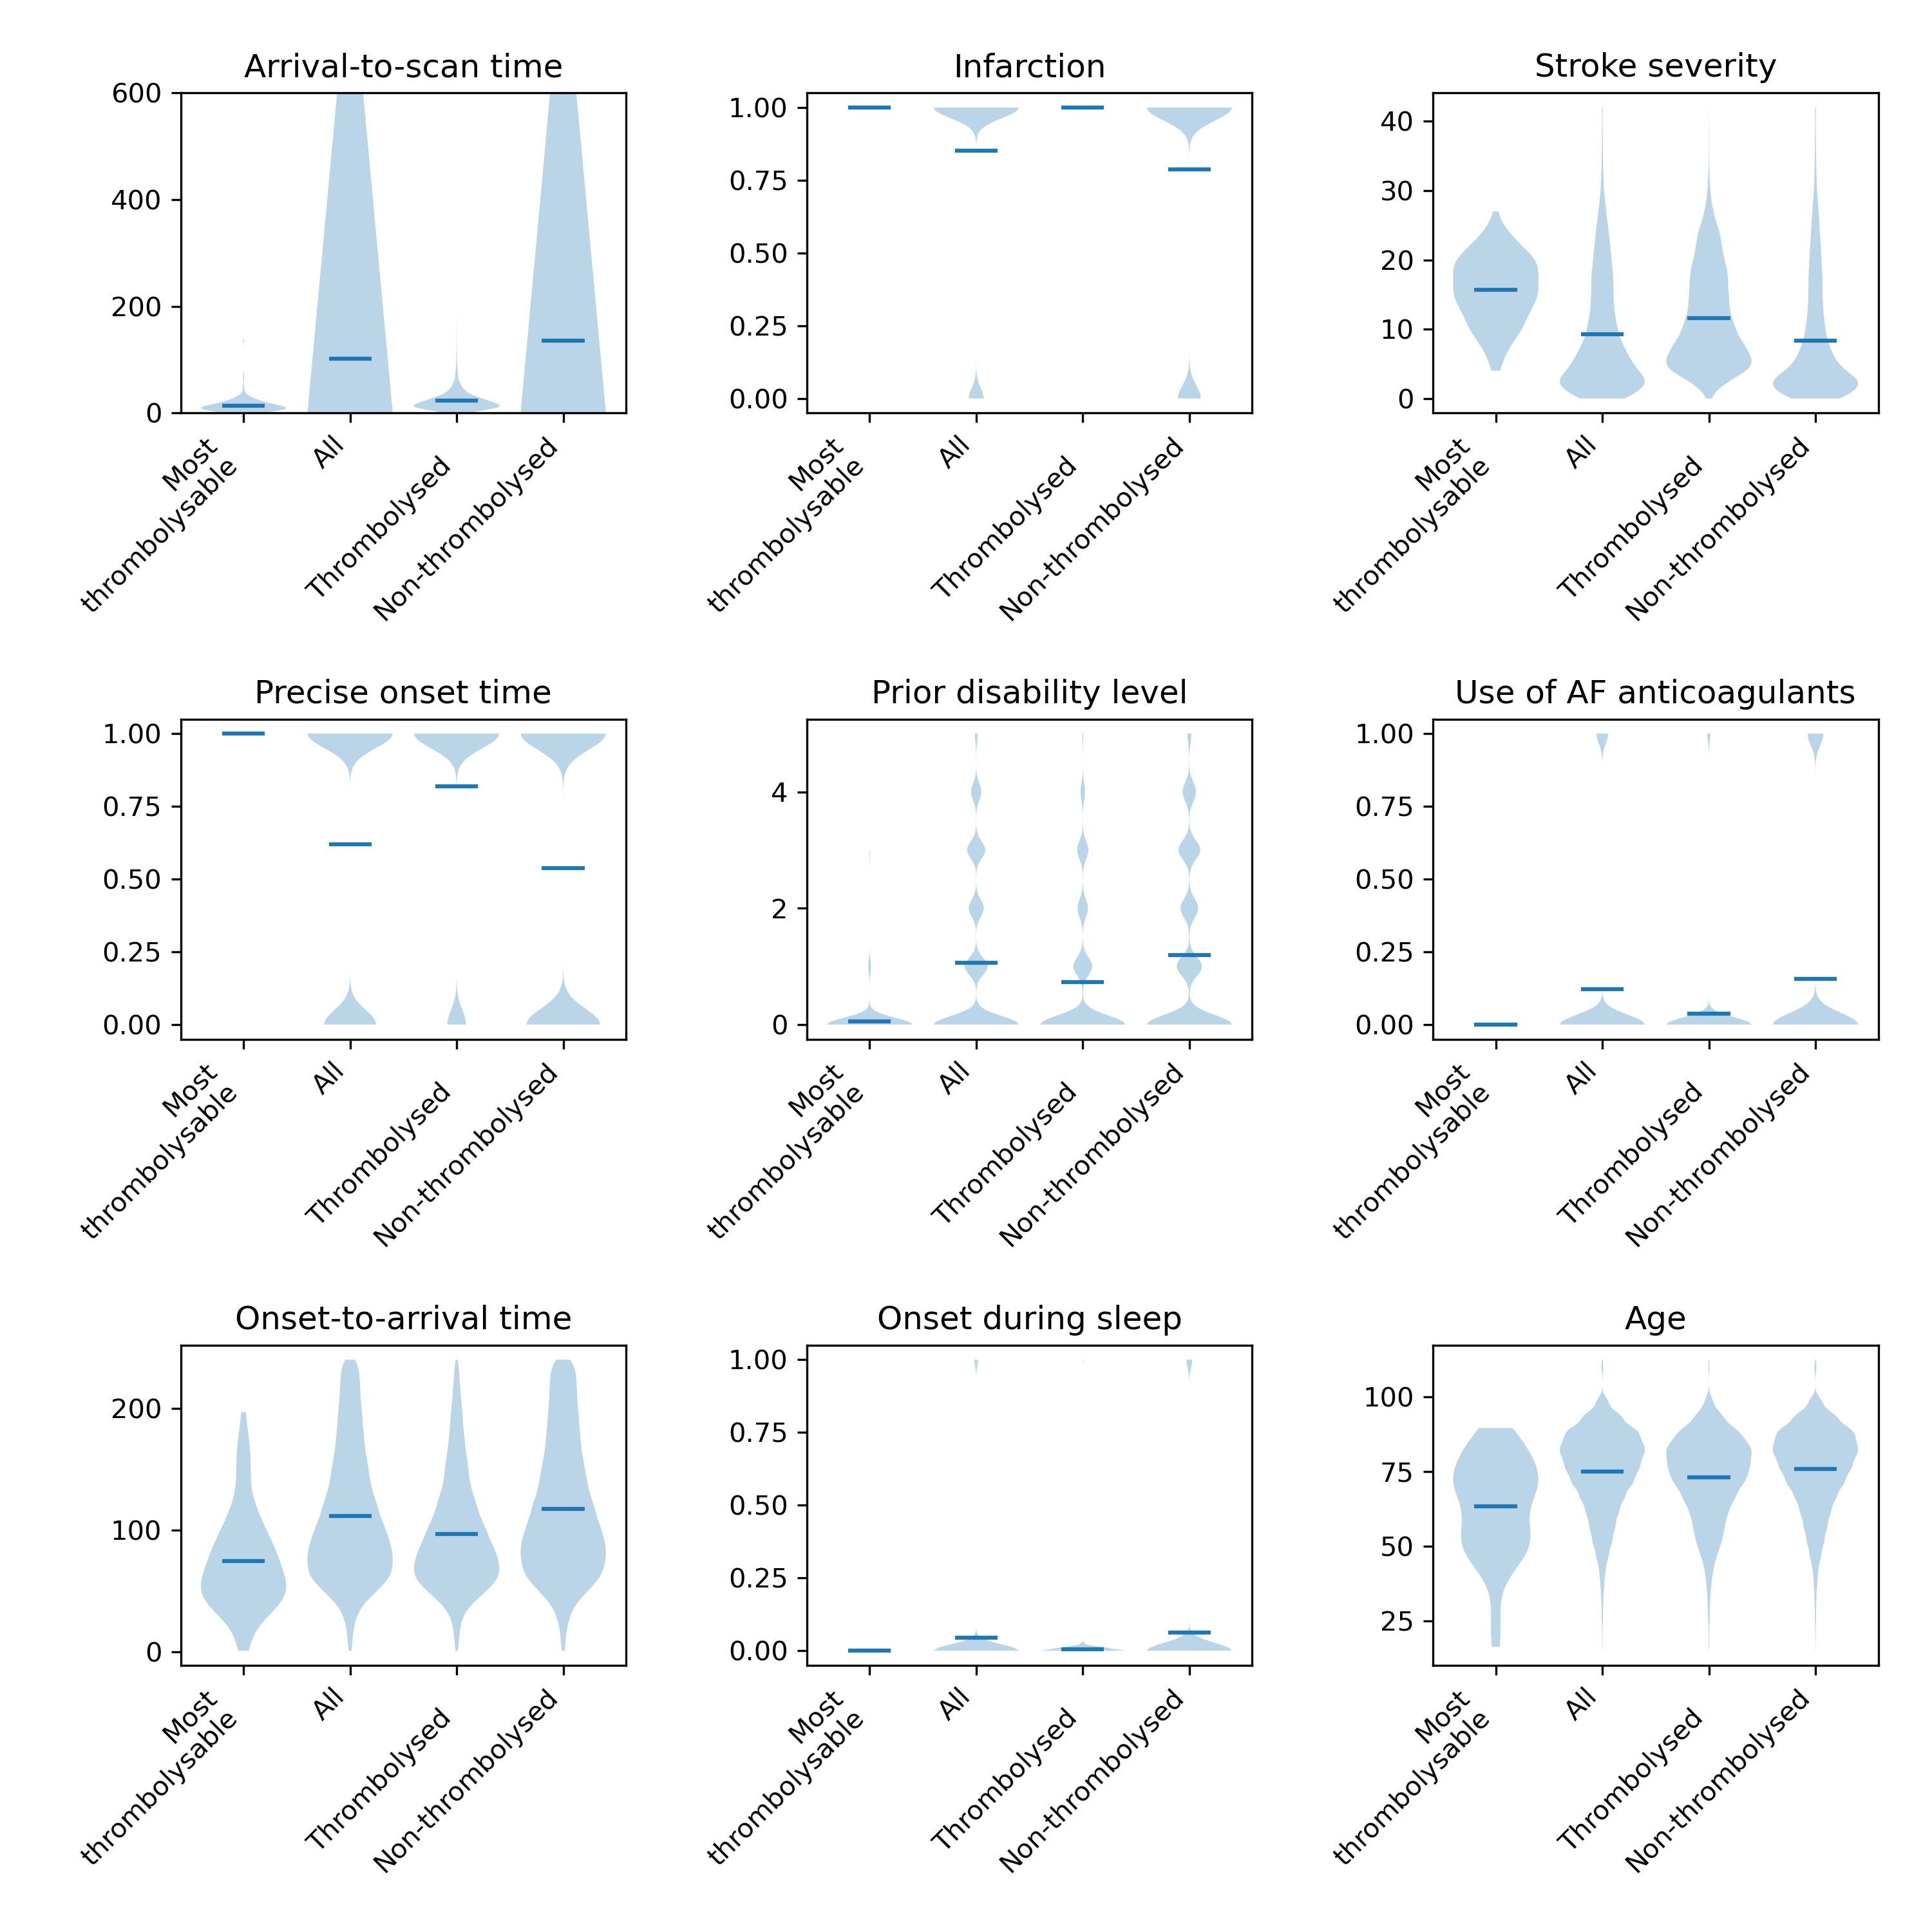
\includegraphics[width=1.0\textwidth]{./images/02a_most_thrombolsyable_violin}
\caption{Violin plots comparing feature values between the patient with the highest probability of thrombolysis at each hospital (`Most thrombolysable') with: 1) all patients, 2) all patients who had received thrombolysis, and 3) all patients who had not received thrombolysis. Horizontal lines show the mean value of each group.}
\label{fig:results_most_thrombolysable}
\end{figure}


%%%%%%%%%%%%%%%%%%%%%%%%%%%%%%%%%%%%%%%%%%%%%%%%%%%%%%%%%%%%%%%%%%%%%%%%
\iffalse
\subsection{Variation in hospital thrombolysis use for patient subgroups}

Figure \ref{fig:results_boxplot} shows a boxplot of observed and predicted use of thrombolysis, broken down by subgroup. The three subgroups of patients with one non-ideal feature (NIHSS $<$5, estimated stroke onset time, pre-stroke mRS $>2$) all had reduced thrombolysis use, and combining these non-ideal features reduced thrombolysis use further. The observed and predicted thrombolysis use show the same general results, but some small differences existed: 1) The use of thrombolysis in \emph{ideal} patients is a little lower in the observed vs predicted results (mean hospital thrombolysis use = 89\% vs 99\%), 2) The predicted results show a stronger effect of combining non-ideal features, 3) The observed thrombolysis rate shows higher between-hospital variation than the predicted thrombolysis rate. This may be partly explained by the observed thrombolysis rate being based on different patients at each hospital, but may also be partly explained by actual use of thrombolysis being slightly more variable than predicted thrombolysis use (which will follow general hospital patterns, and will not include, for example, between-clinician variation at each hospital).

For both the predicted and observed thrombolysis, subgroup thrombolysis use tended to reduce in parallel (r-squared 0.221 to 0.308 in observed thrombolysis use, and 0.445 to 0.621 in the predicted thrombolysis use). \kpFIXME{State reduce, but these values increase}

\begin{figure}[!h]
\centering
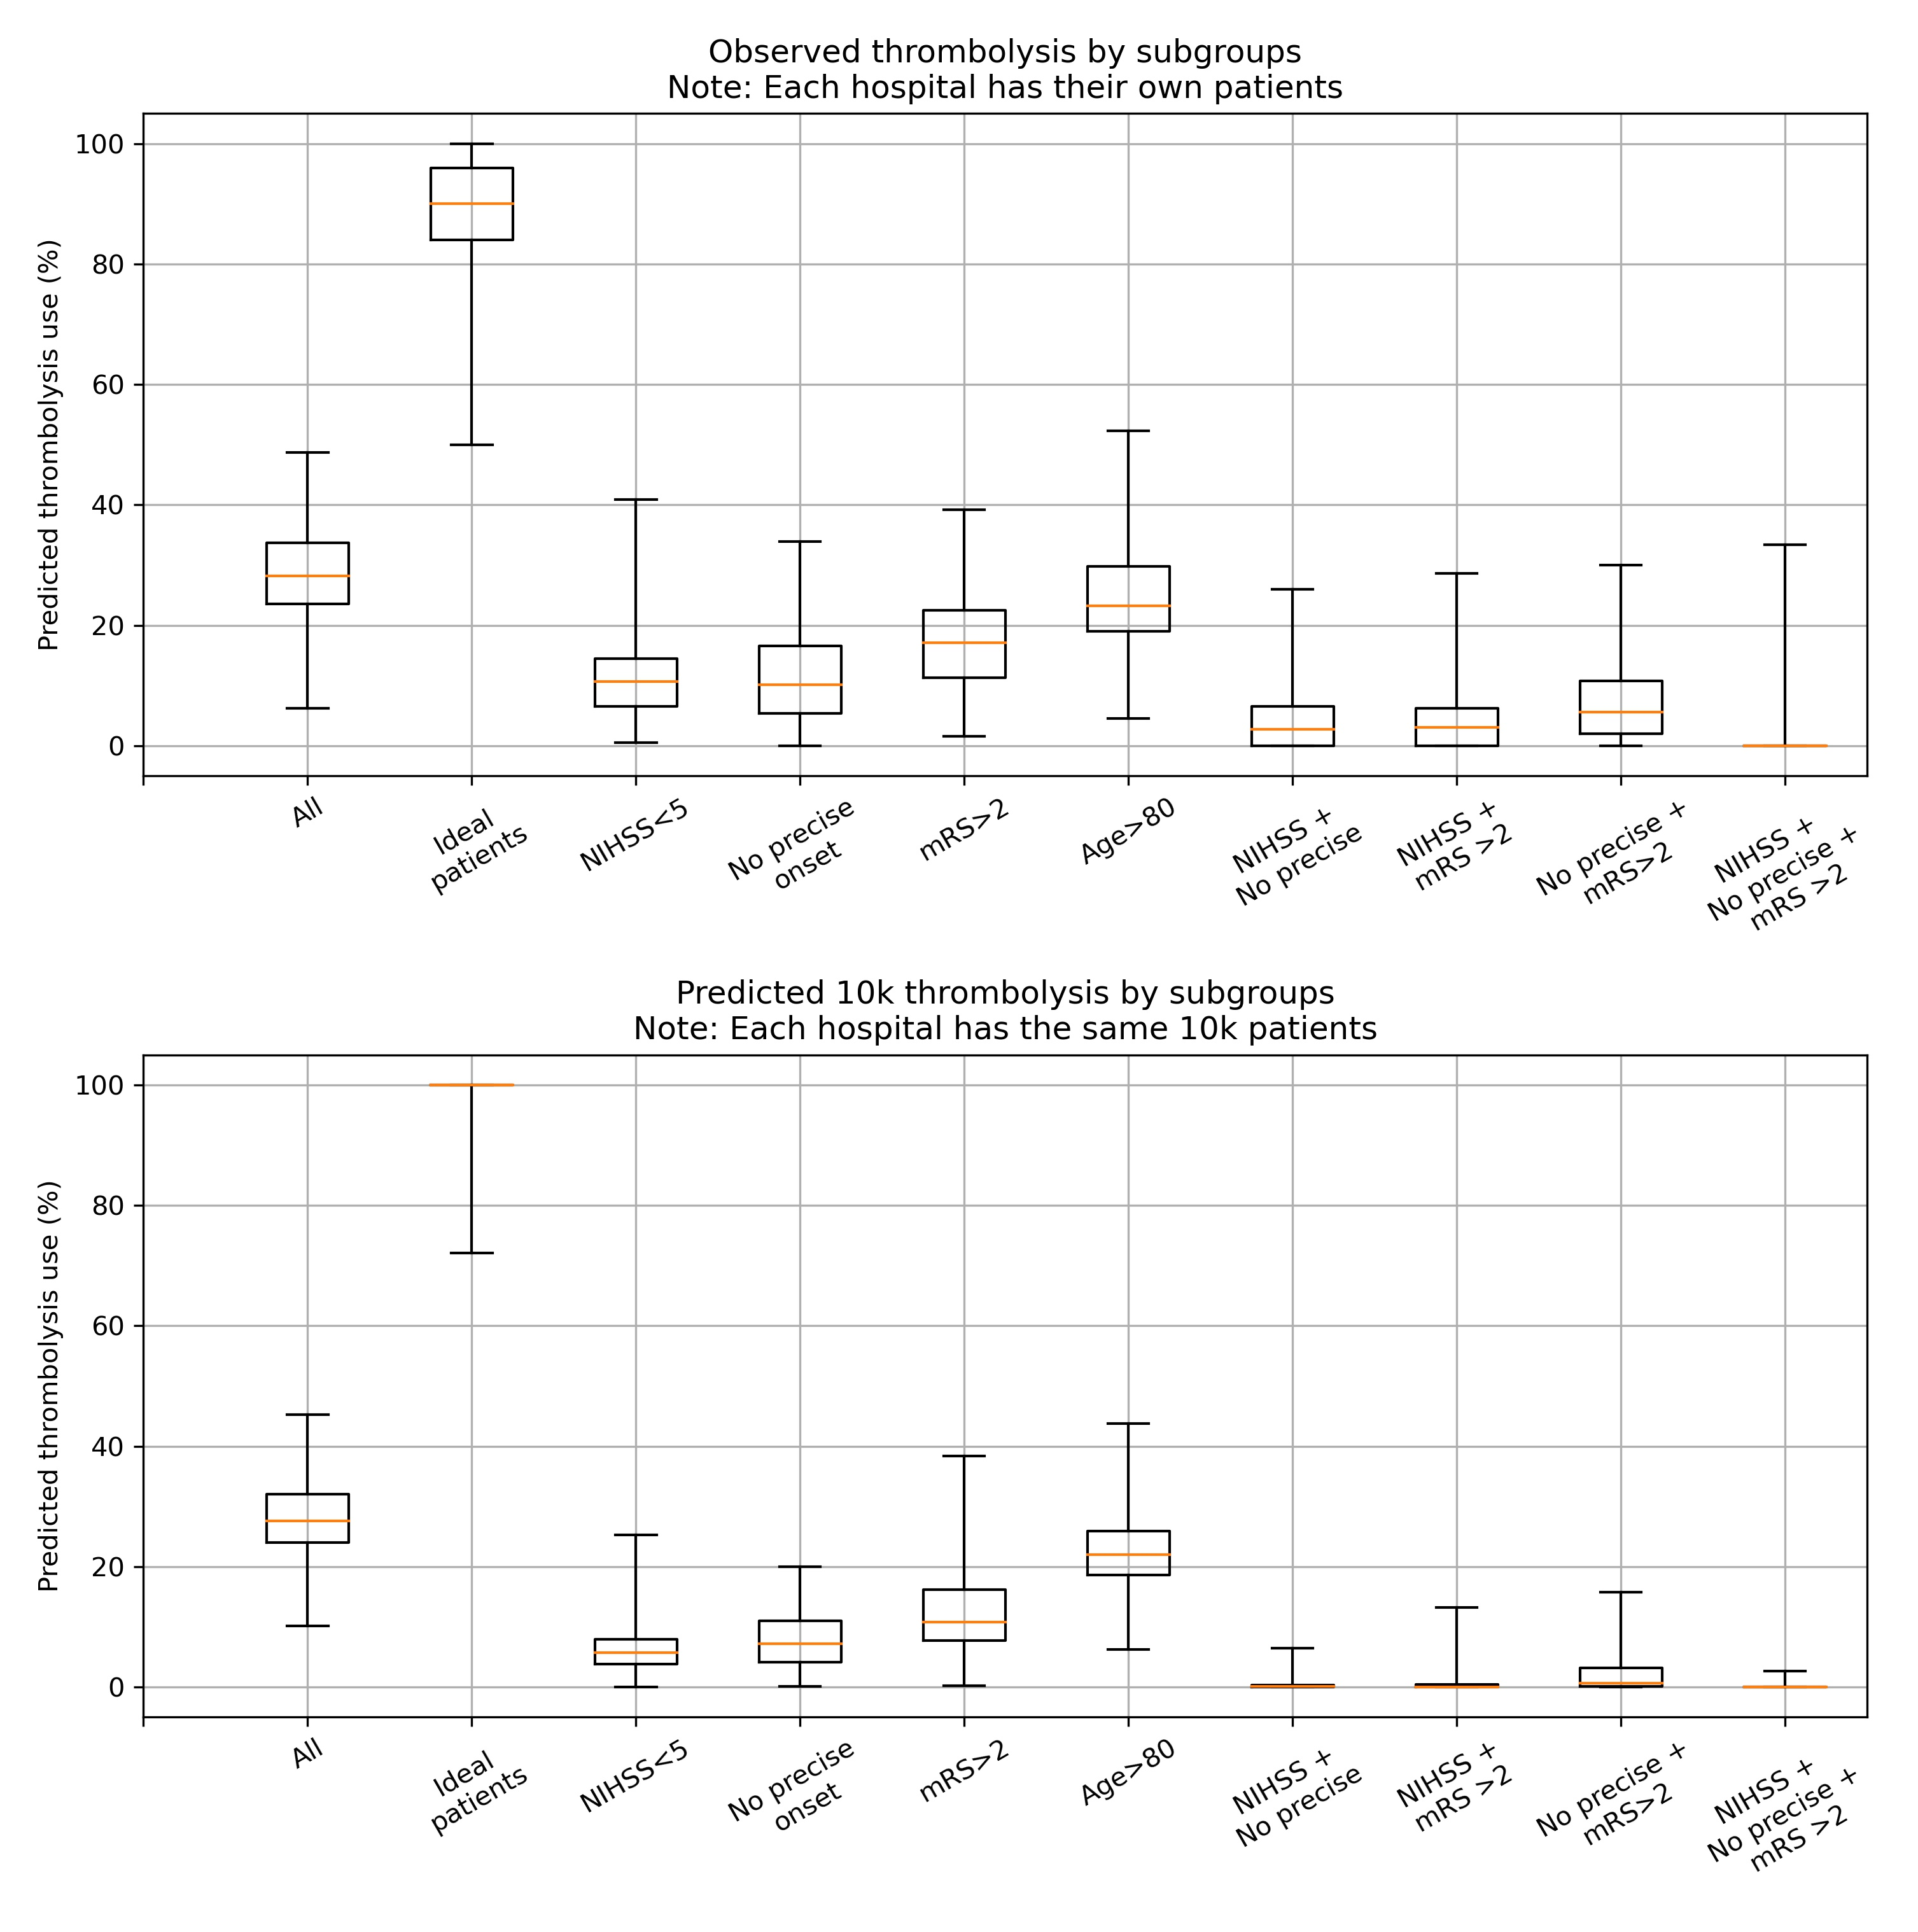
\includegraphics[width=1\textwidth]{./images/15a_actual_vs_modelled_subgroup_violin}
\caption{Boxplot for either observed (top) or predicted (bottom) use of thrombolysis for subgroups of patients.}
\label{fig:results_boxplot}
\end{figure}
\fi
%%%%%%%%%%%%%%%%%%%%%%%%%%%%%%%%%%%%%%%%%%%%%%%%%%%%%%%%%%%%%%%%%%%%%%%%

\subsection{Individual patient SHAP values}
SHAP values are presented as how they affect log odds of receiving thrombolysis, but for individual predictions, probability values are more intuitive. Figure \ref{fig:results_waterfall} shows waterfall plots for an example of a patient with low (top) and high (bottom) probability of receiving thrombolysis. Waterfall plots show the influence of features for an individual prediction (in our case, patient). The SHAP model starts with a base prediction of a 24\% probability of receiving thrombolysis, before feature values are taken into account. For the patient with a low probability of receiving thrombolysis, the two most influential features reducing the probability of receiving thrombolysis were a long arrival-to-scan time (138 minutes) and a low stroke severity (NIHSS=2). For the patient with a high probability of receiving thrombolysis, the two most influential features increasing the probability of receiving thrombolysis were a short arrival-to-scan time (17 minutes) and a moderate stroke severity (NIHSS=14). 

\begin{figure}[!h]
\centering
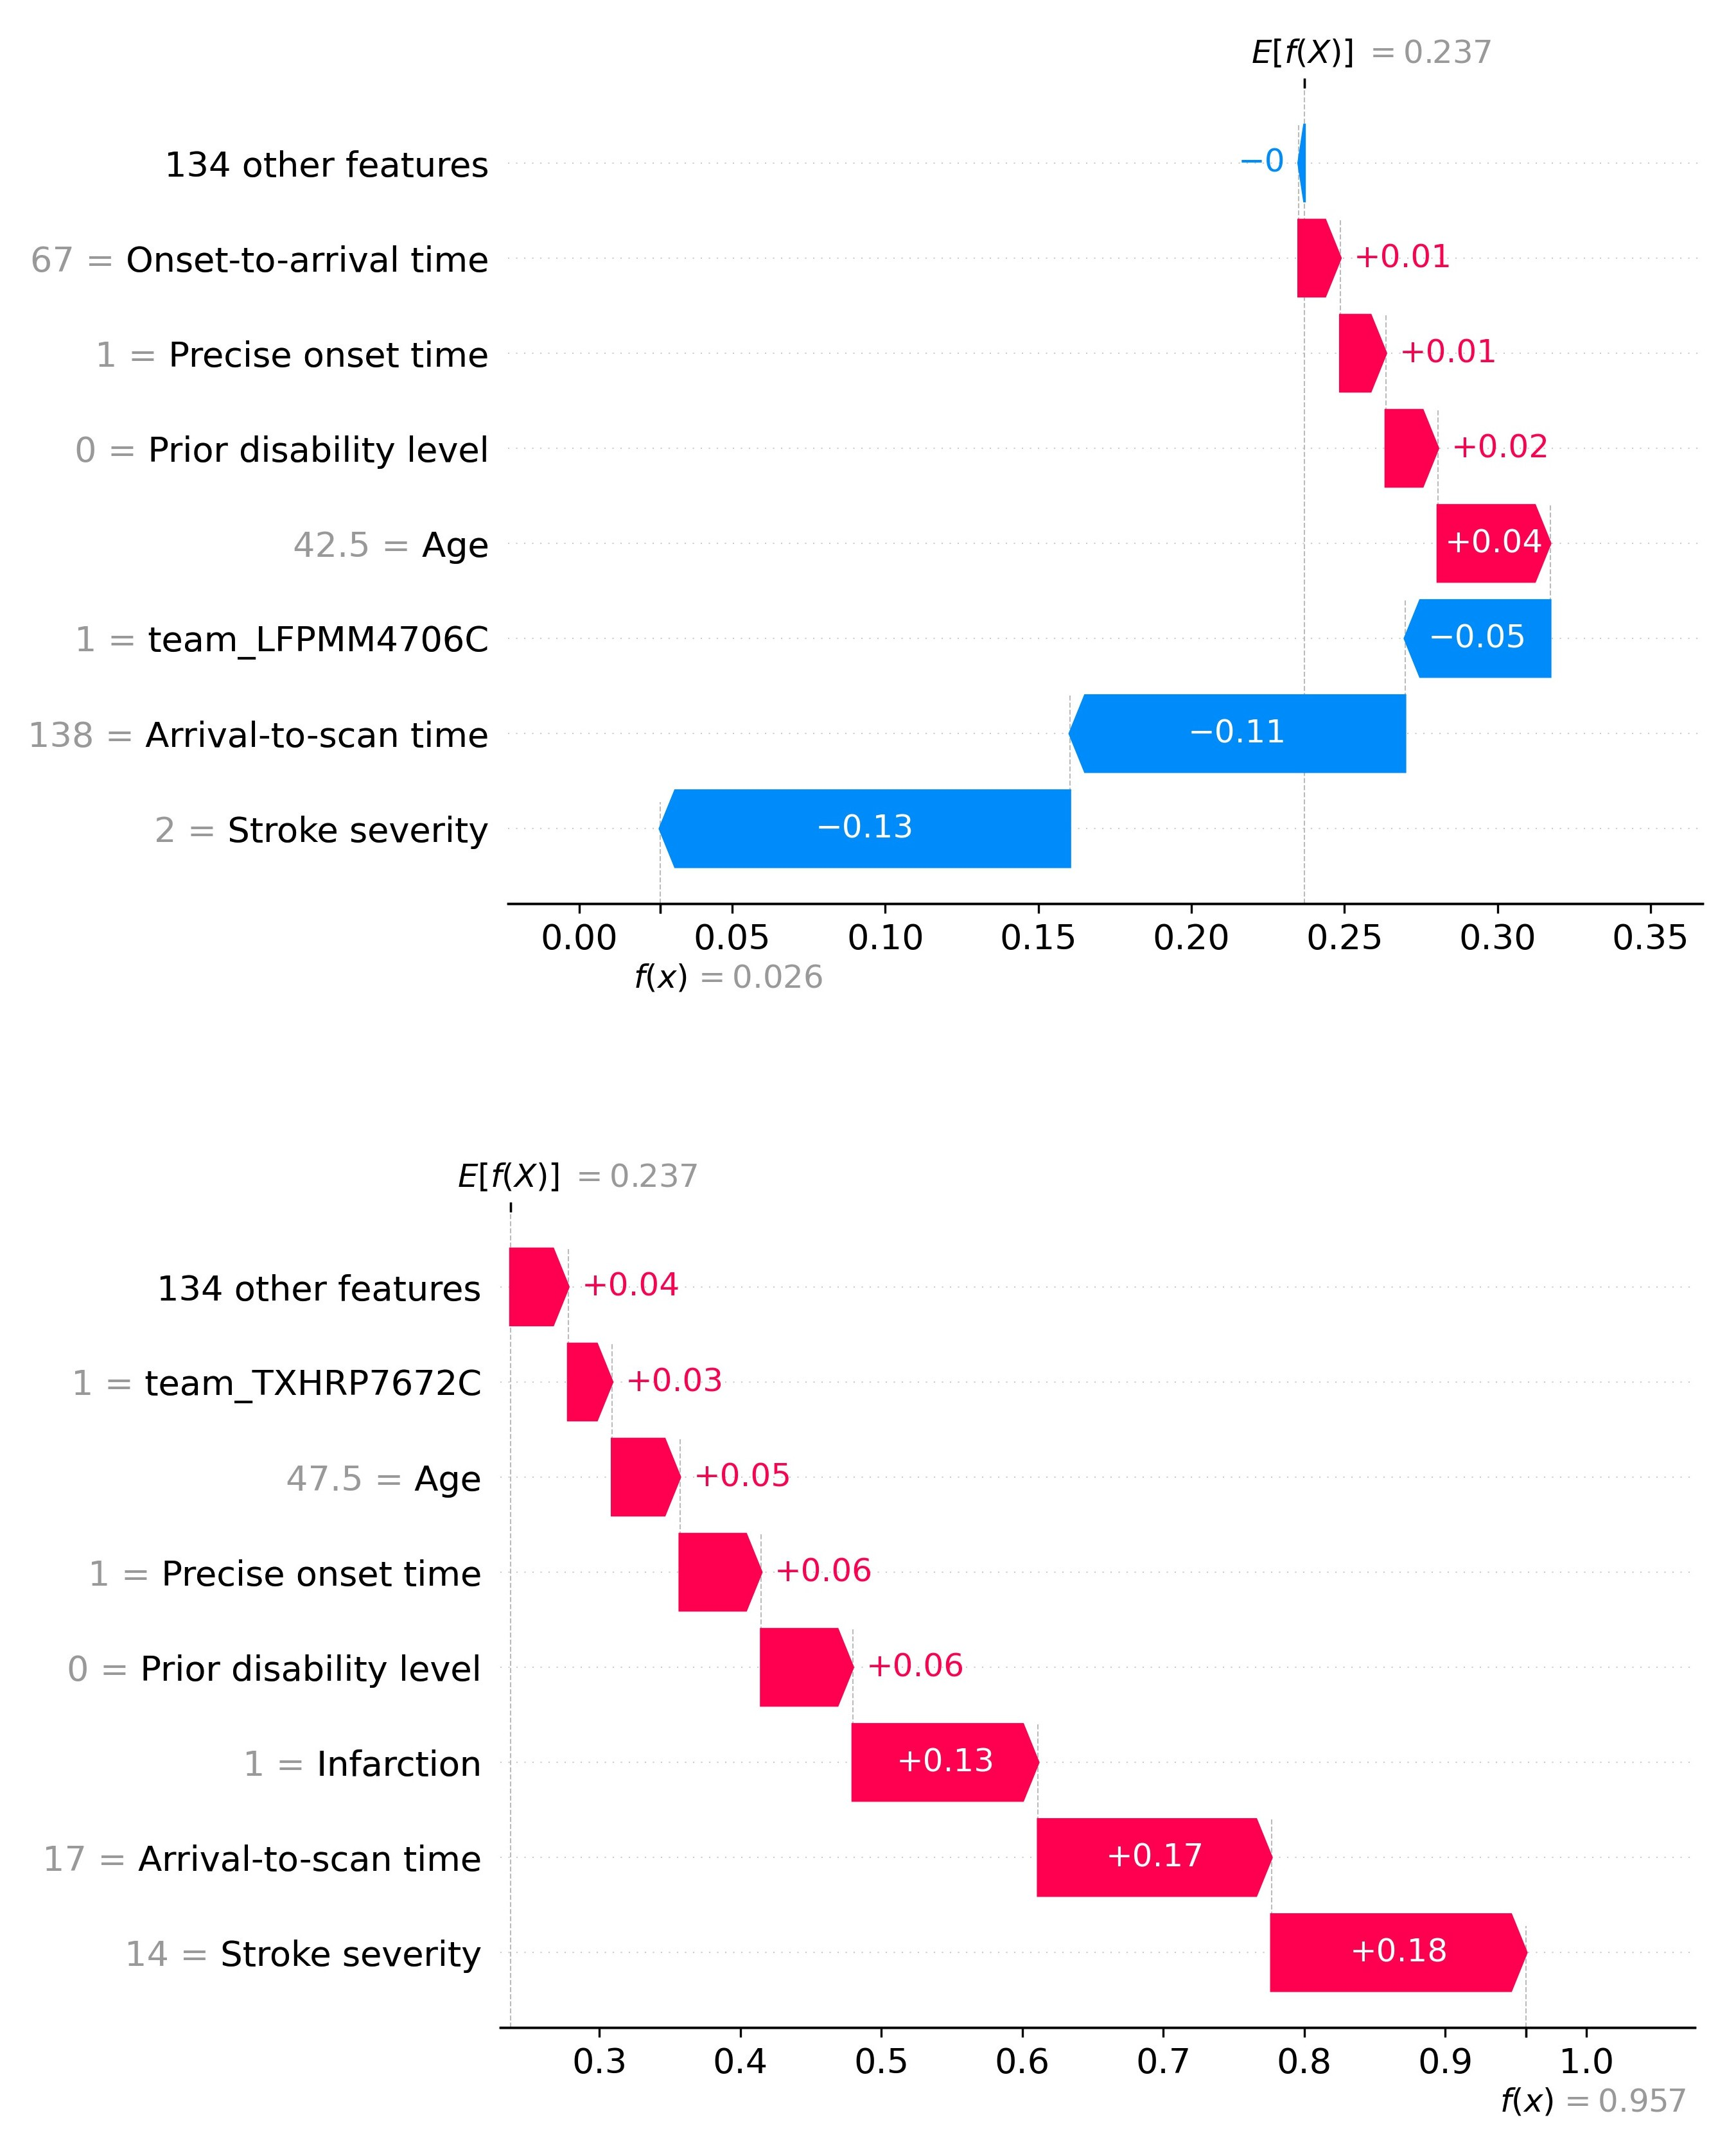
\includegraphics[width=0.8\textwidth]{./images/waterfall}
\caption{Waterfall plots showing the influence of each feature on the predicted probability of a single patient receiving thrombolysis. Top: An example of a patient with a low probability (2.6\%) of receiving thrombolysis. Bottom: An example of a patient with a high probability (95.7\%) of receiving thrombolysis.}
\label{fig:results_waterfall}
\end{figure}


%%%%%%%%%%%%%%%%%%%%%%%%%%%%%%%%%%%%%%%%%%%%%%%%%%%%%%%%%%%%%%%%%%%%%%%%

\subsection{The relationship between feature values and the odds of receiving thrombolysis (SHAP values)}

Figure \ref{fig:results_shap_violin} shows the relationship between feature values and SHAP values for the top six influential features, for the 71,142 individual patients in the first of the 5 k-fold training set. Key observations are (with SHAP influence converted from log-odds to odds):

\begin{itemize}
    \item \emph{Stroke type}: The SHAP values for stroke type show that the model effectively eliminated any probability of receiving thrombolysis for non-ischaemic (haemorrhagic) stroke.
    \item \emph{Arrival-to-scan time}: The odds of receiving thrombolysis reduced by about 20 fold over the first 100 minutes of arrival to scan time.
    \item \emph{Stroke severity (NIHSS)}: The odds of receiving thrombolysis were lowest at NIHSS 0, increased and peaked at NIHSS 15-25, and then fell again with higher stroke severity (NIHSS above 25). The difference between minimum odds (at NIHSS 0) and maximum odds (at 15-25) of receiving thrombolysis was 30-35 fold.
    \item \emph{Stroke onset time type (precise vs. estimated)}: The odds of receiving thrombolysis were about 3 fold greater for precise onset time than estimated onset time.
    \item \emph{Disability level (mRS) before stroke}: The odds of receiving thrombolysis fell about 5 fold between mRS 0 and 5.
\end{itemize}


\begin{figure}[!h]
\centering
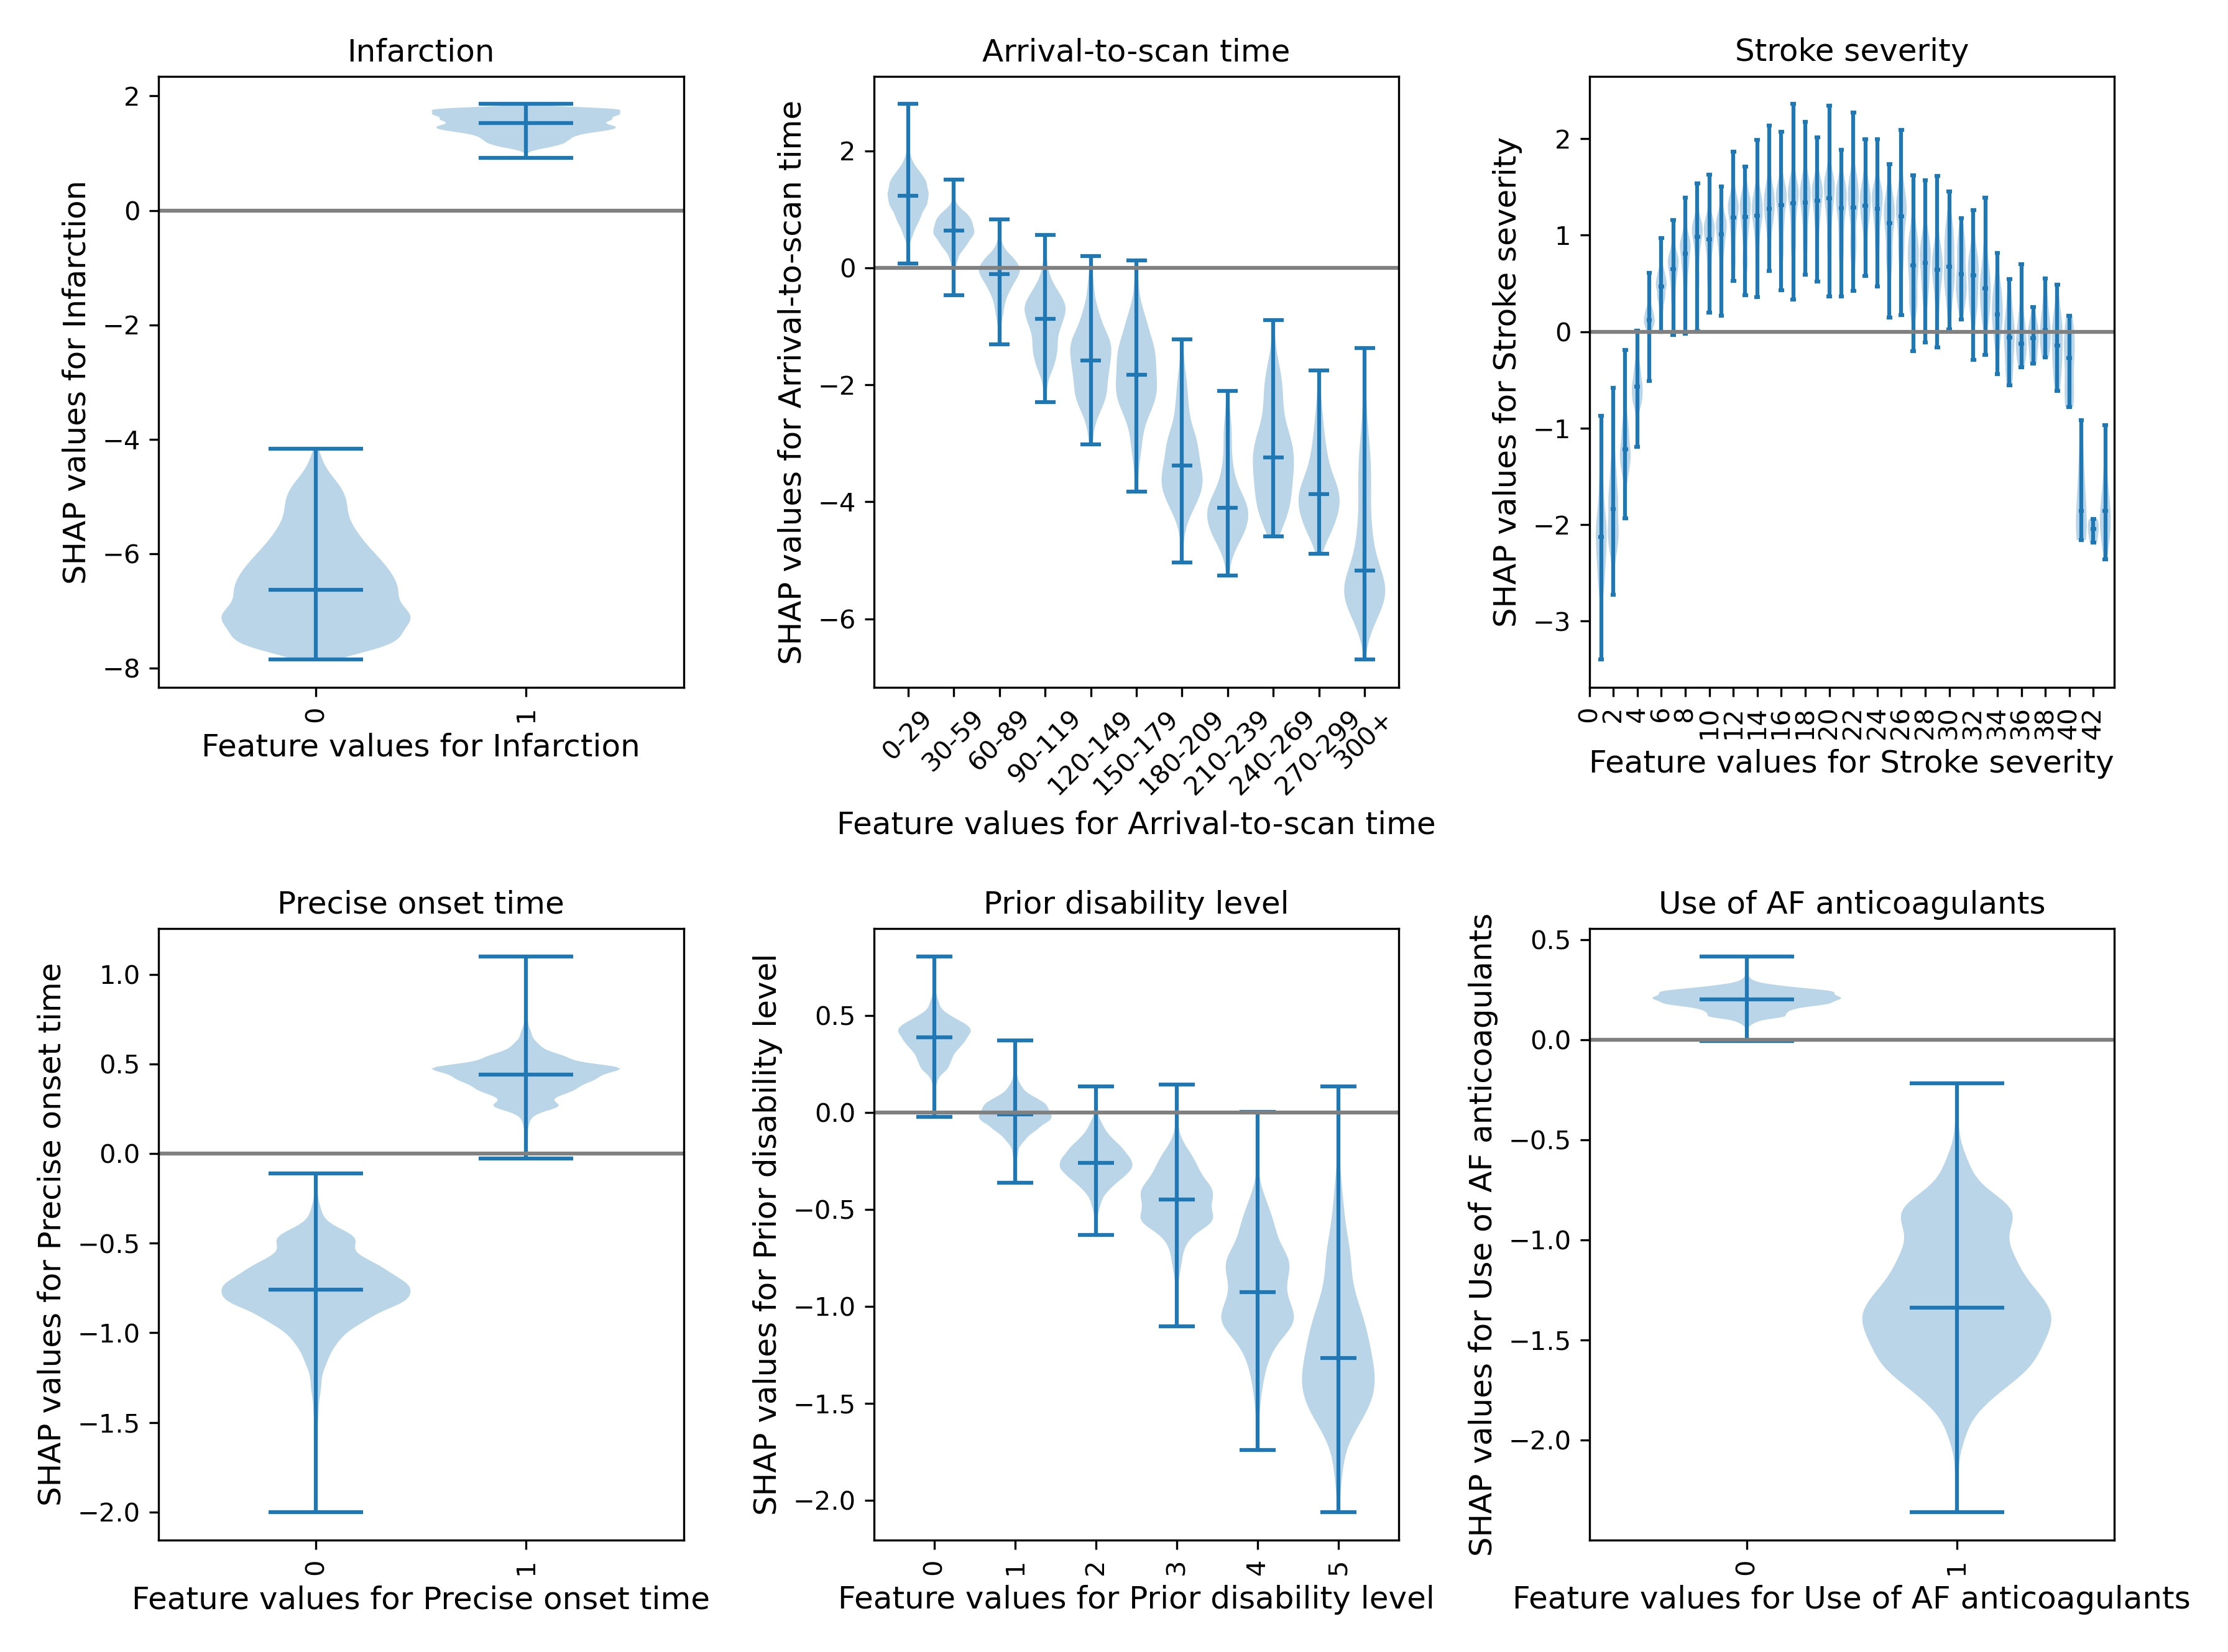
\includegraphics[width=1\textwidth]{./images/03_xgb_10_features_thrombolysis_shap_violin}
\caption{Violin plots showing the relationship between SHAP values and feature values. The horizontal line shows the median SHAP value. SHAP values were taken from the 71,142 patients in the first of the 5 k-fold training set.}
\label{fig:results_shap_violin}
\end{figure}

%%%%%%%%%%%%%%%%%%%%%%%%%%%%%%%%%%%%%%%%%%%%%%%%%%%%%%%%%%%%%%%%%%%%%%%%

\subsection{How the hospital SHAP value compares with the hospitals use of thrombolysis}

Using the \emph{all data model}, the hospital SHAP values ranged from -1.4 to +1.4 (for patients attending each hospital). This range of SHAP (log odds) represented a 15 fold difference in odds of receiving thrombolysis between hospitals (most were in the range of -1 to +1, but this still represents a 7-8 fold difference in odds of receiving thrombolysis).

The median hospital SHAP value correlated with the observed hospital thrombolysis rate with an r-squared of 0.582, suggesting that 58\% (P$<$0.0001) of the between-hospital variance in thrombolysis use may be explained by the hospitals' SHAP values, i.e. the hospitals' predisposition and/or preparedness to use thrombolysis.

Using the \emph{10k holdout model}, the predicted use of thrombolysis across the 132 hospitals for the identical 10k cohort of patients (not used in training the model) ranged from 10\% to 45\%. The median hospital SHAP value for the 10k cohort of patients correlated very closely with the predicted thrombolysis use in the 10k cohort of patients at each hospital (r-squared = 0.944), confirming that the hospital SHAP is providing a direct insight into a hospitals' propensity to use thrombolysis.

%to predict between-hospital differences in use of thrombolysis if all hospitals had the same patients arriving. All patient feature values were kept constant, except the hospital coding was changed to mimic all patients attending each of the 132 hospitals. P
%%%%%%%%%%%%%%%%%%%%%%%%%%%%%%%%%%%%%%%%%%%%%%%%%%%%%%%%%%%%%%%%%%%%%%%%

\subsection{How individual hospitals may modify general patterns of thrombolysis}

%The main effect of having a precise onset time was to increase the odds of receiving thrombolysis, as indicated by a positive SHAP value. Individual hospitals (in addition to the hospital feature having it's own main effect of influencing the odds of receiving thrombolysis) has their pair-wise interaction effect with each feature, such as on the effect of having a precise onset time. The top line of graphs in Figure \ref{fig:results_shap_hosp_intercations} show that some hospitals (such as "FAJKD7118X") attenuate the main effect, leading to a smaller difference in odds of receiving thrombolysis, whereas some hospitals (such as "HZNVT9936G") strengthening the effect, leading to a larger difference in odds of receiving thrombolysis depending on whether stroke onset time is known precisely.

The main effect of having a precise onset time was to increase the odds of receiving thrombolysis, as indicated by a positive SHAP value. Hospitals have a direct effect on the odds of receiving thrombolysis (as seen in the SHAP main effect for the hospital feature), but they may also modify the effect of other features. The top line of graphs in Figure \ref{fig:results_shap_hosp_intercations} show that some hospitals (such as \emph{FAJKD7118X}) attenuate the effect of knowing stroke onset time precisely, leading to a smaller difference in odds of receiving thrombolysis, whereas some hospitals (such as \emph{HZNVT9936G}) strengthening the effect, leading to a larger difference in odds of receiving thrombolysis depending on whether stroke onset time is known precisely.

The plots in the first column of Figure \ref{fig:results_shap_hosp_intercations} shows the main effect for three features (precise onset time, stroke severity, and prior disability), followed by examples of hospitals which either attenuated (column two) or strengthened (column three) the effect of those three features. These SHAP interactions revealed how individual hospitals may differ in how they modify the effect of other patient features.

\begin{figure}[!h]
\centering
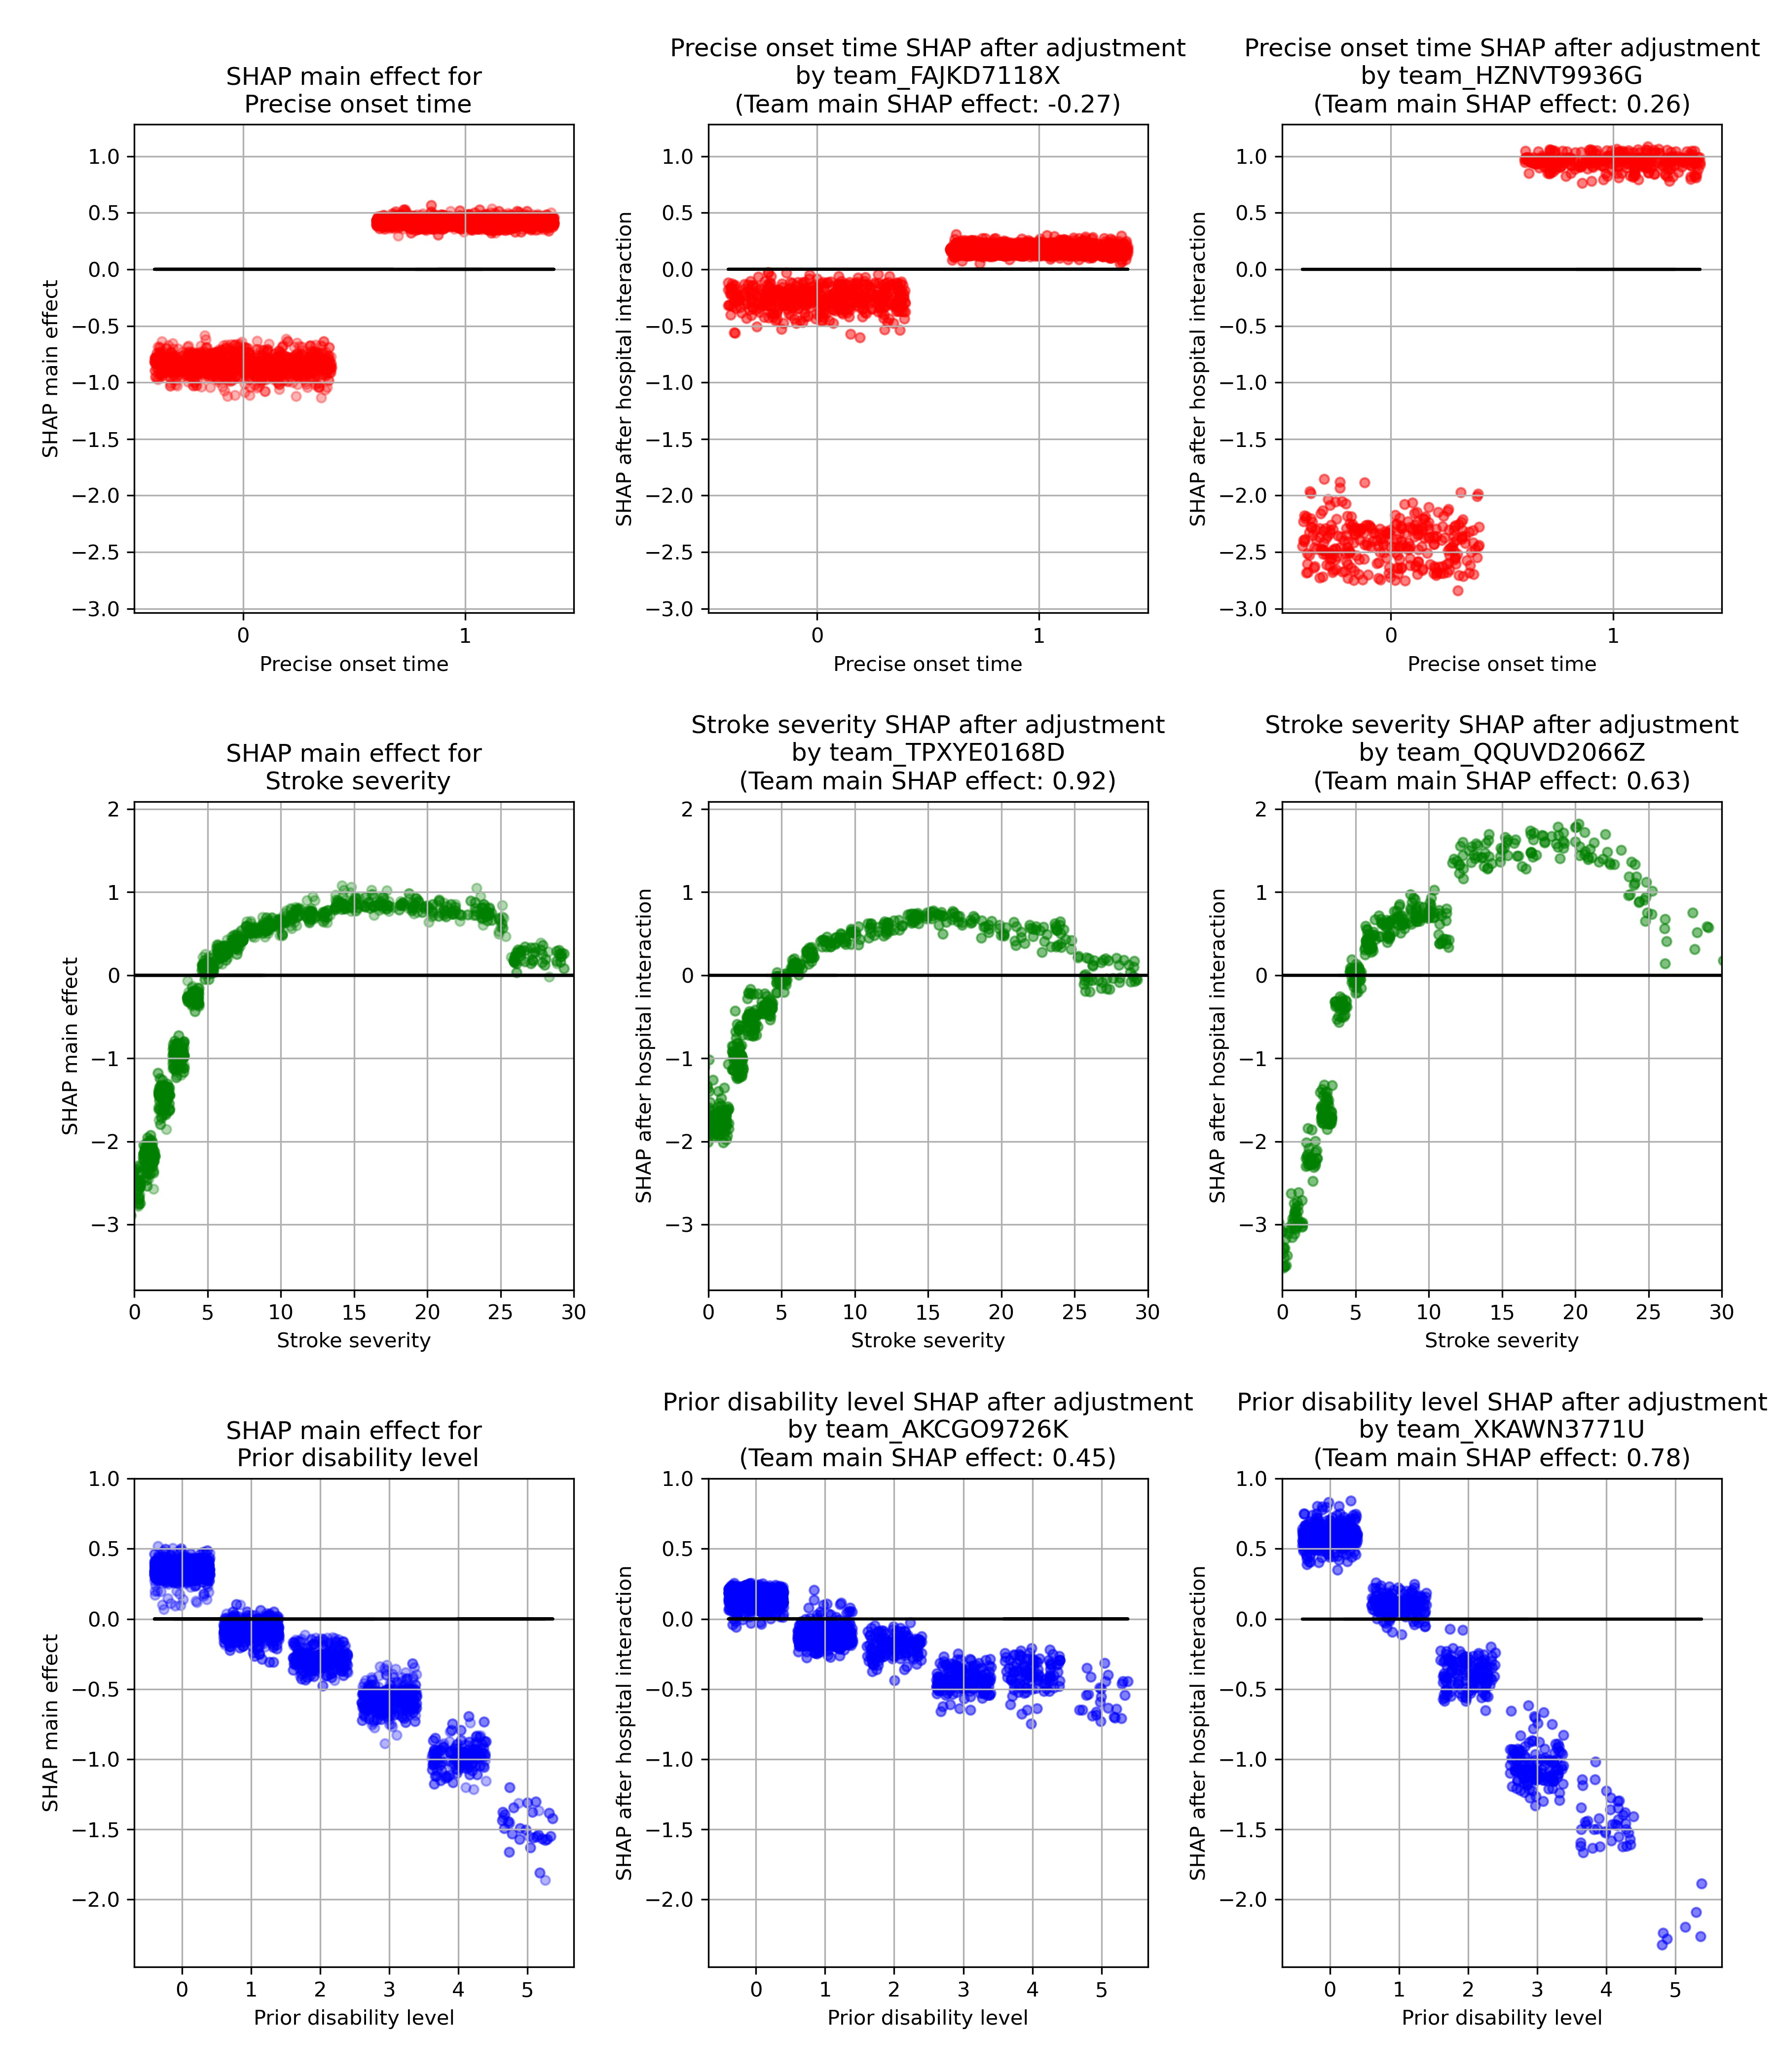
\includegraphics[width=1.0\textwidth]{./images/12aa_three_way_shap_adjustment}
\caption{Adjustment of SHAP main effects by individual hospital. Each row first (left) shows the SHAP main effect of the feature, then (middle) a hospital where the SHAP interaction attenuates the main effect, and finally (right) a hospital where the SHAP interaction strengthens the main effect. Top row (red): SHAP main effect and adjusted SHAP values for precise stroke onset time. Middle row (green): SHAP main effect and adjusted SHAP values for stroke severity. Bottom row (blue): SHAP main effect and adjusted SHAP values for pre-stroke disability.}
\label{fig:results_shap_hosp_intercations}
\end{figure}
%%%%%%%%%%%%%%%%%%%%%%%%%%%%%%%%%%%%%%%%%%%%%%%%%%%%%%%%%%%%%%%%%%%%%%%%%%%%%%%%%%%%%%%%%%%%%

\subsection{Comparing predicted thrombolysis decisions across hospitals, using artificial patients}

Our artificial \emph{ideally thrombolysable patient} was predicted to receive thrombolysis at 131/132 hospitals. By just changing two of the patients characteristics to create our artifical \emph{likely thrombolysable patient} (from a stroke severity of NIHSS 15 to 5, and from a precise to an estimated stroke onset time), that patient would be expected to receive thrombolysis in only 35\% of hospitals. To further explore this between hospital variation, Figure \ref{fig:results_artifical_shap_waterfall_with_violin} shows how the model predicts how each of the 132 hospitals responds to each of the \emph{likely thrombolysable patients} feature values, to arrive at the individual probability of receiving thrombolysis at each of the 132 hospitals (3 - 88\%).

\begin{figure}[!h]
\centering
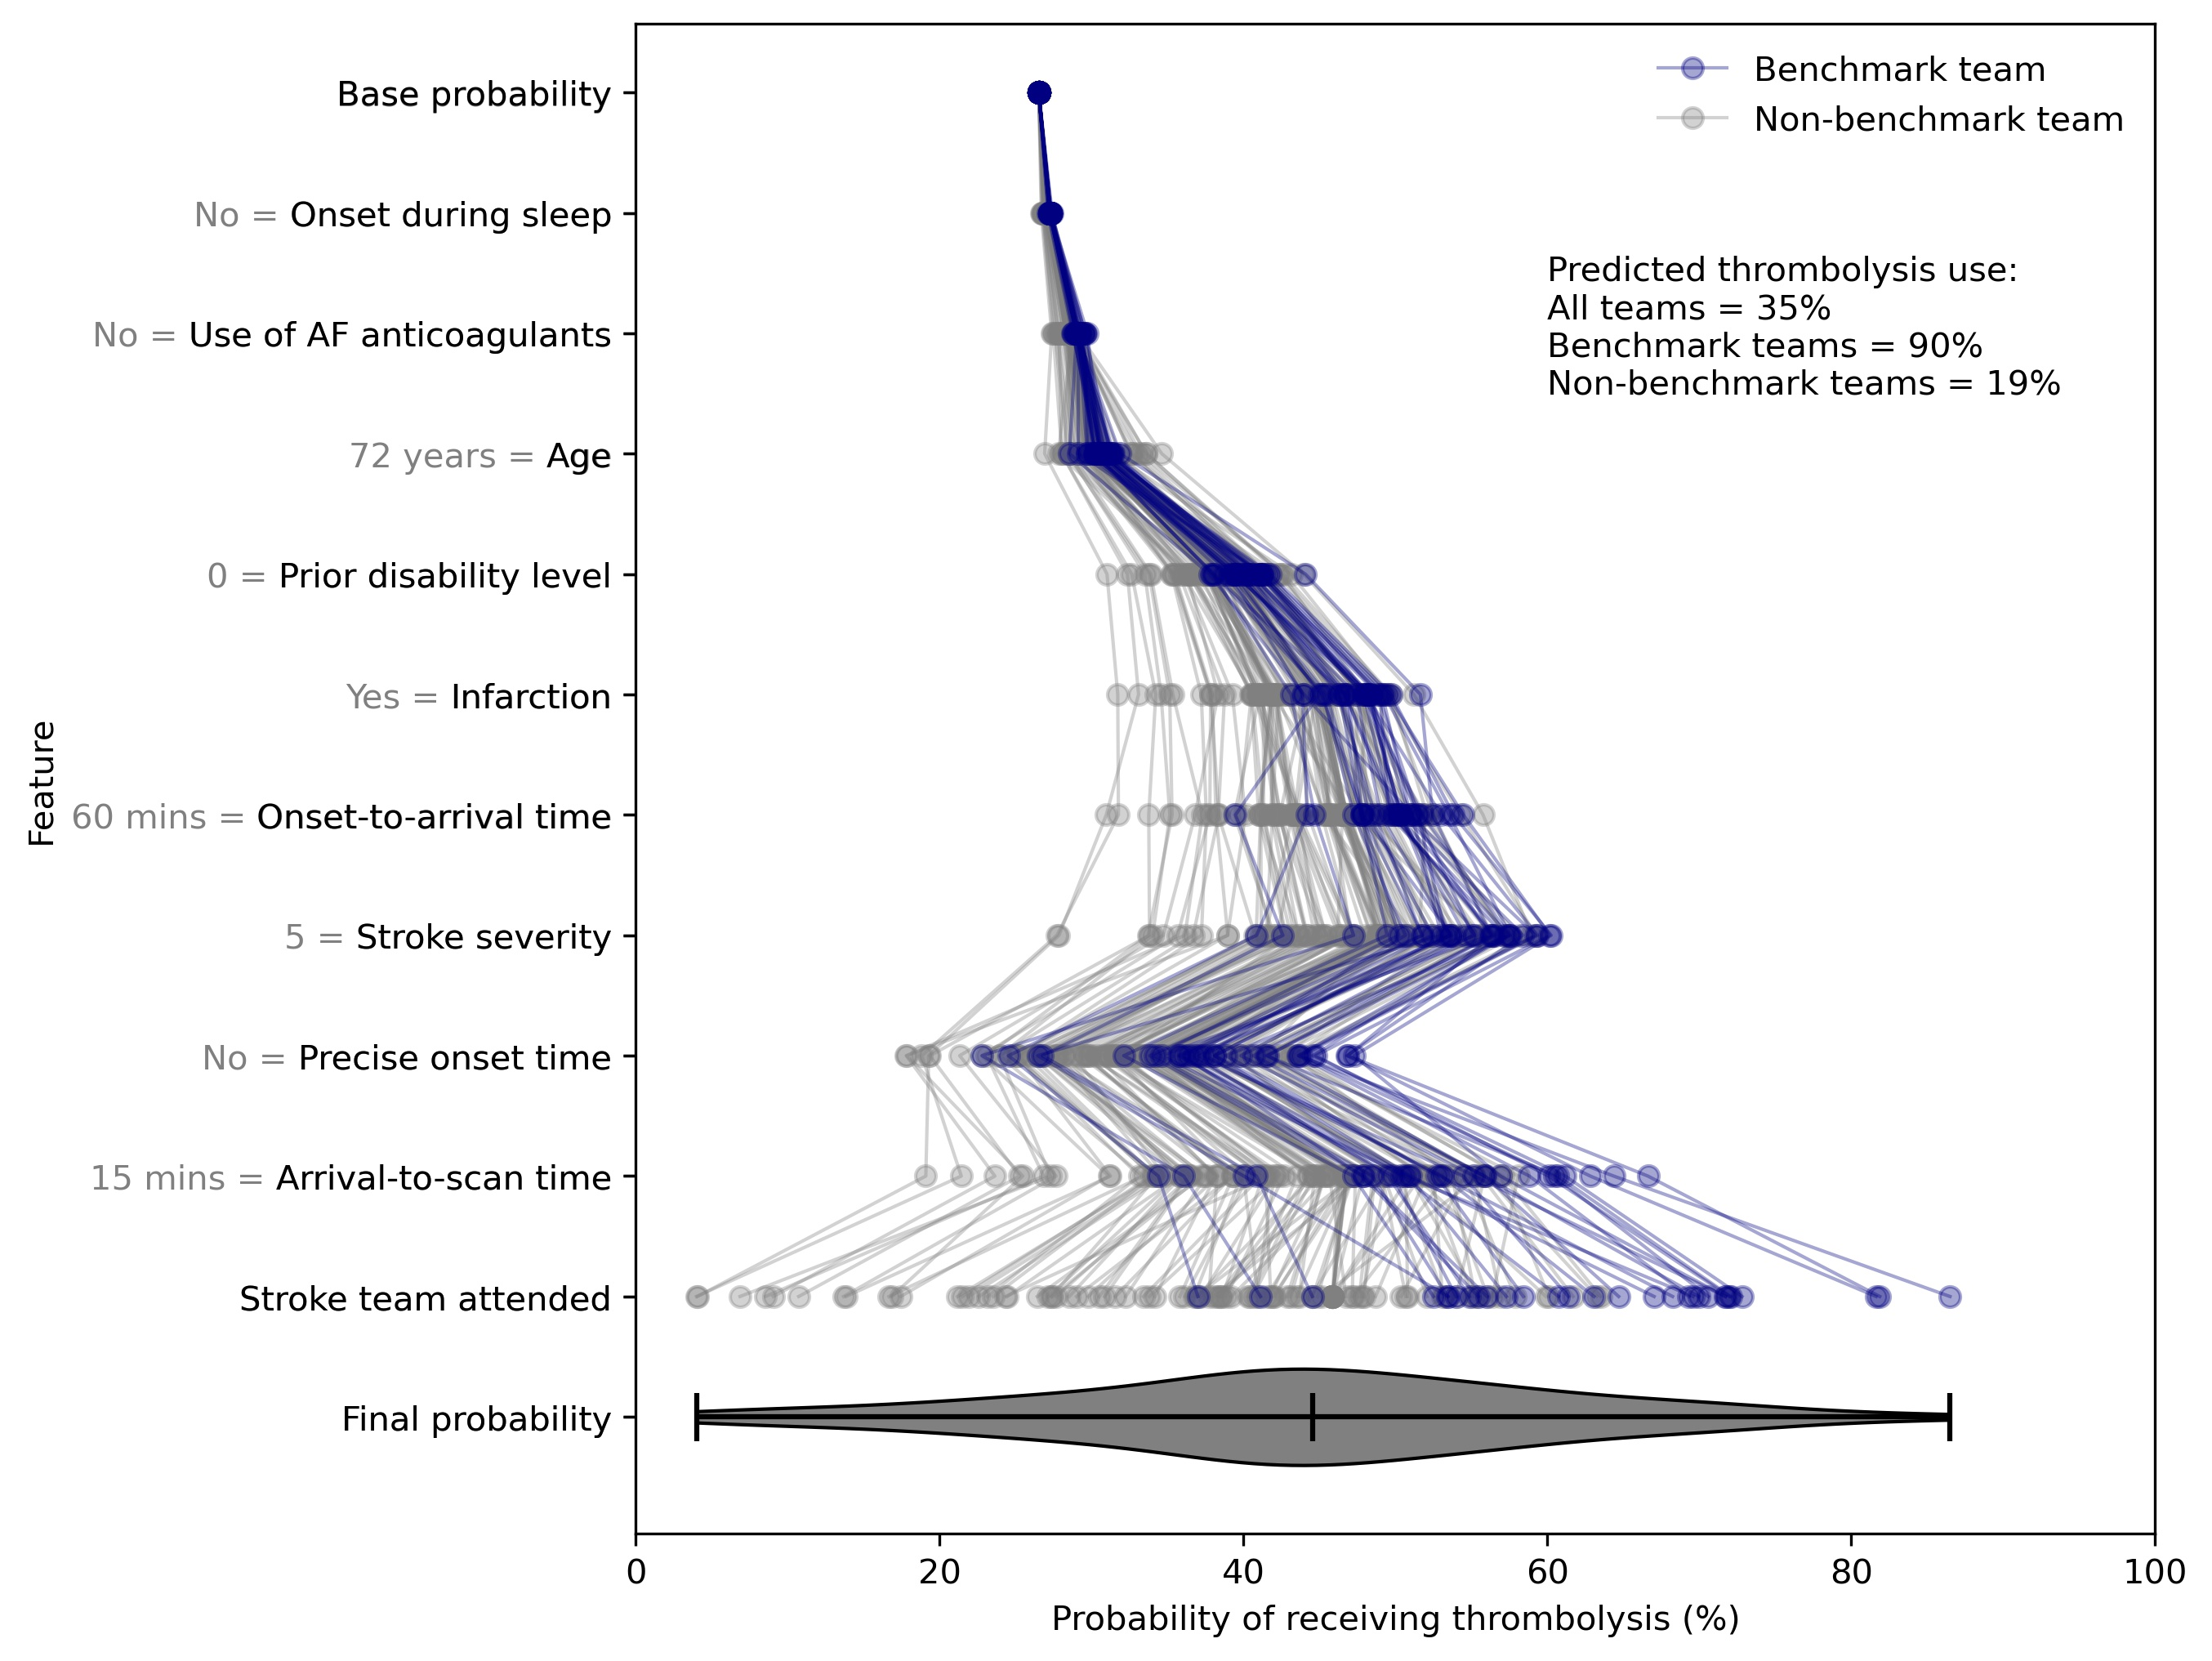
\includegraphics[width=0.85\textwidth]{./images/21_shap_waterfall_with_violin_contentious}
\caption{SHAP plots for the same patient attending 132 different hospitals. The patient has the following feature values: Onset to arrival = 60 mins, Arrival to scan = 15 mins, Infarction = 1, NIHSS = 5, Prior disability level = 0, Precise onset time = 0, Use of AF anticoagulants = 0. The plot shows how each patient feature value contributes to the final prediction of whether that patients is likely to receive thrombolysis.}
\label{fig:results_artifical_shap_waterfall_with_violin}
\end{figure}








